\section{Resultater fra Affinity diagram}
\label{ParametreDatabehandlingAffinityDiagram}
%
%Den her sektion skal indeholde vores analyse af vores affinity diagram, samt billeder af det. 
%
Da formålet med projektet er, at udlede hvilke parametre danske rejsende tilskriver interaktionen med en social robot for efterfølgende at udvikle skalaer, som kan bruges til evaluere oplevelsen af interaktionen med robotten, bør der fremsættes nogle krav for hvordan parametrene udvælges for dernæst at formulere dem til skalaer. 

For at udlede parametrene fokuseres der på én grøn kategori af gangen, hvorfra parametrene formuleres på baggrund af både pink og blå labels. Parametrene vil formuleres som et udsagn, der kan evalueres på en skala, hvorfor parametre noteres med et \textit{S} på en orange \textit{sticky note}. De orange \textit{sticky notes} kan derudover indeholde design idéer \textit{DI}, indsigter \textit{I} samt idéer til det efterfølgende testdesign \textit{TD}. \blankline
%Skriv om de kriterier, de orange post its er formuleret ud fra. Skriv hvilke kriterier vi så vælger de relevante orange post its ud fra. 
%NOGET OM HVORDAN PARAMETRENE ER "FUNDET" 
%
Der blev i alt dannet 50 orange \textit{sticky note}: \\
S (Skala): 42\\
I (Indsigt): 1\\
DI (Design Idé): 6\\
TD (Test Design): 1\\

%Muligvis en eller anden smart oversigt over hvilke parametre vi "ender" med. Jeg ved ikke om det er her skalaerne burde indgå eller om det skal vente til den part, der handler om en næste test. 

\subsection{Interagerer ikke med R}
%
\begin{figure}[H]
\centering
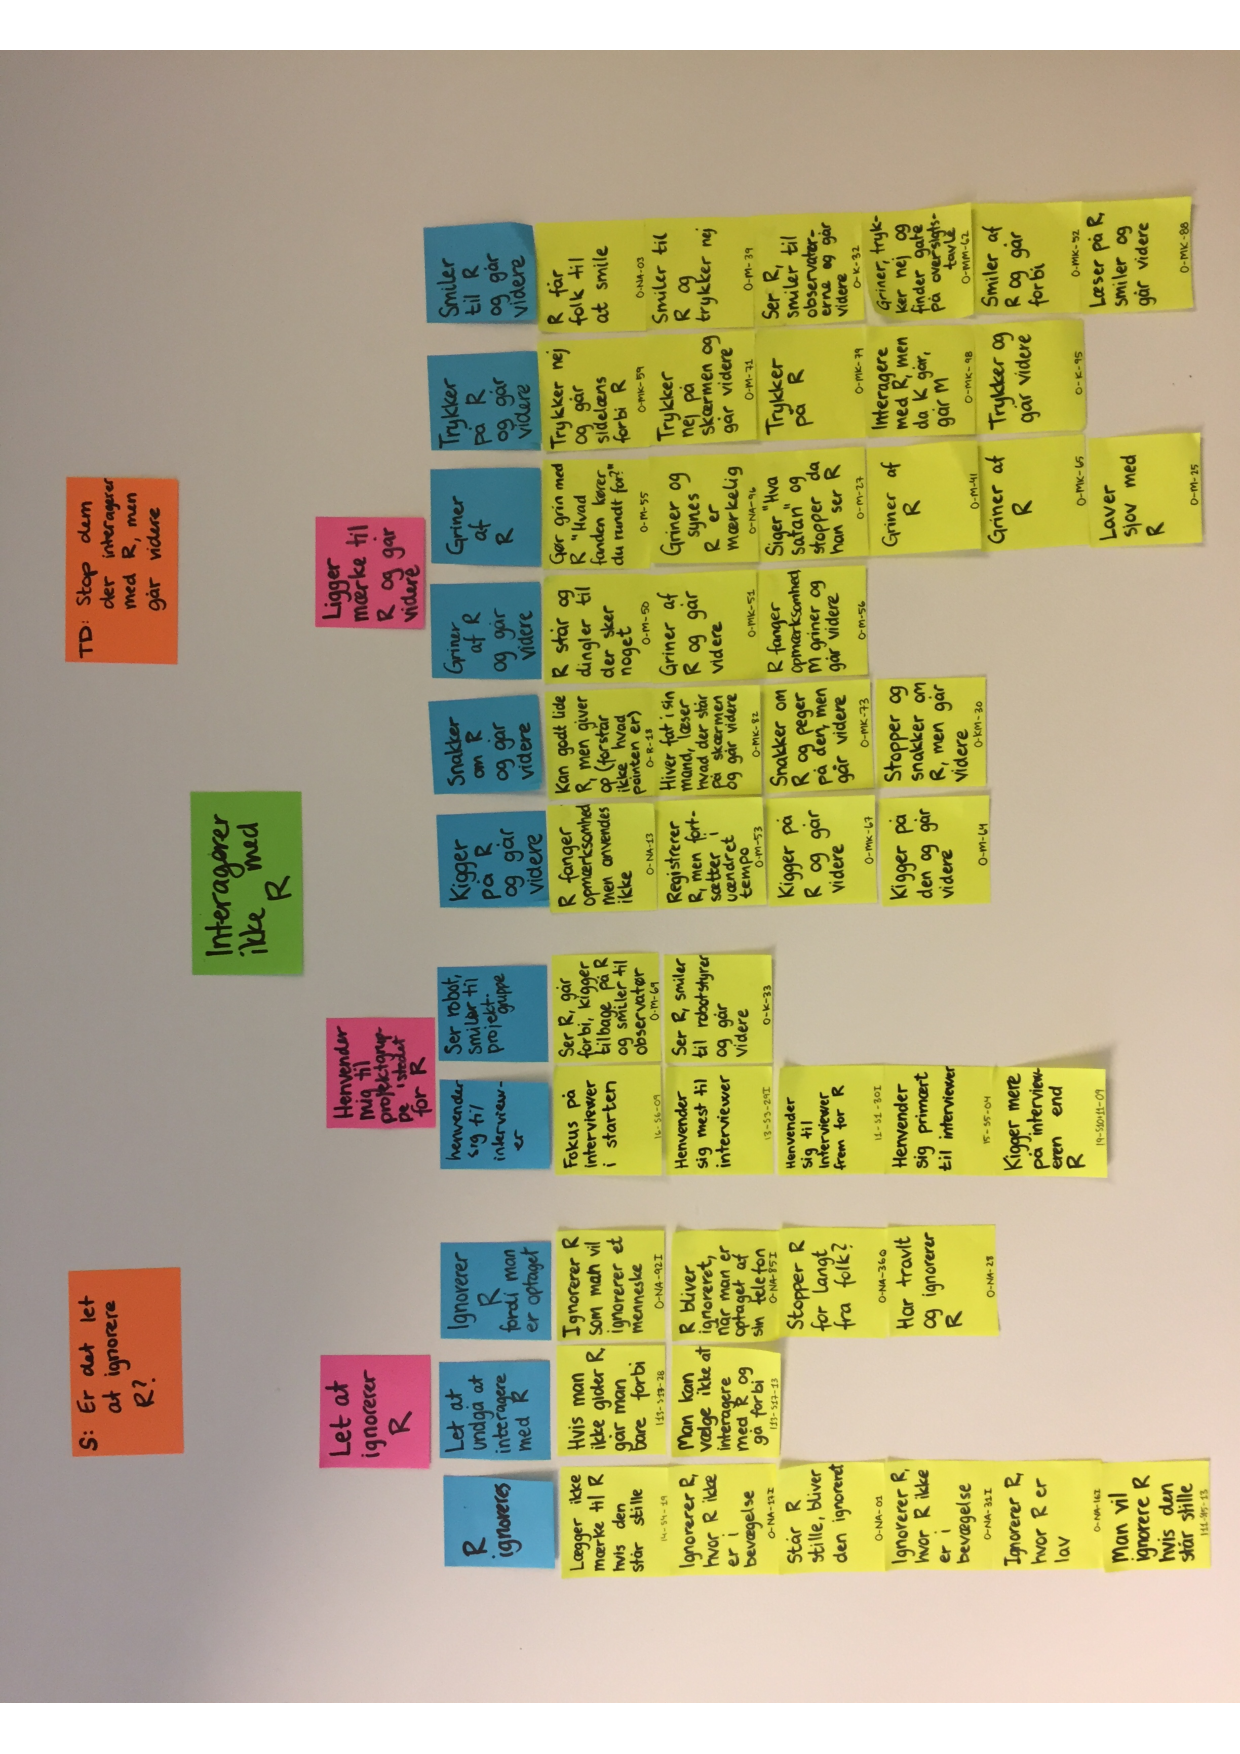
\includegraphics[width = 0.7\textwidth, angle = -90]{Figure/AffinityDiagram/InteragererIkkeMedR} 
\caption{Oversigt over pink, blå og gule \textit{sticky notes} under den overordnede kategori ``Interagerer ikke med R`` samt de udledte parametre på orange \textit{sticky notes}.}
\label{fig:AFInteragererIkkeMedR}
\end{figure}
\noindent
%
S: Er det let at ignorer R?\\
TD: Stop dem der interagerer med R, men går videre. 
%som ikke har lyst til at deltage i interviewet og spørg hvorfor de ikke har lyst til at deltage. 
\subsection{Skærmen virker ikke}
%
\begin{figure}[H]
\centering
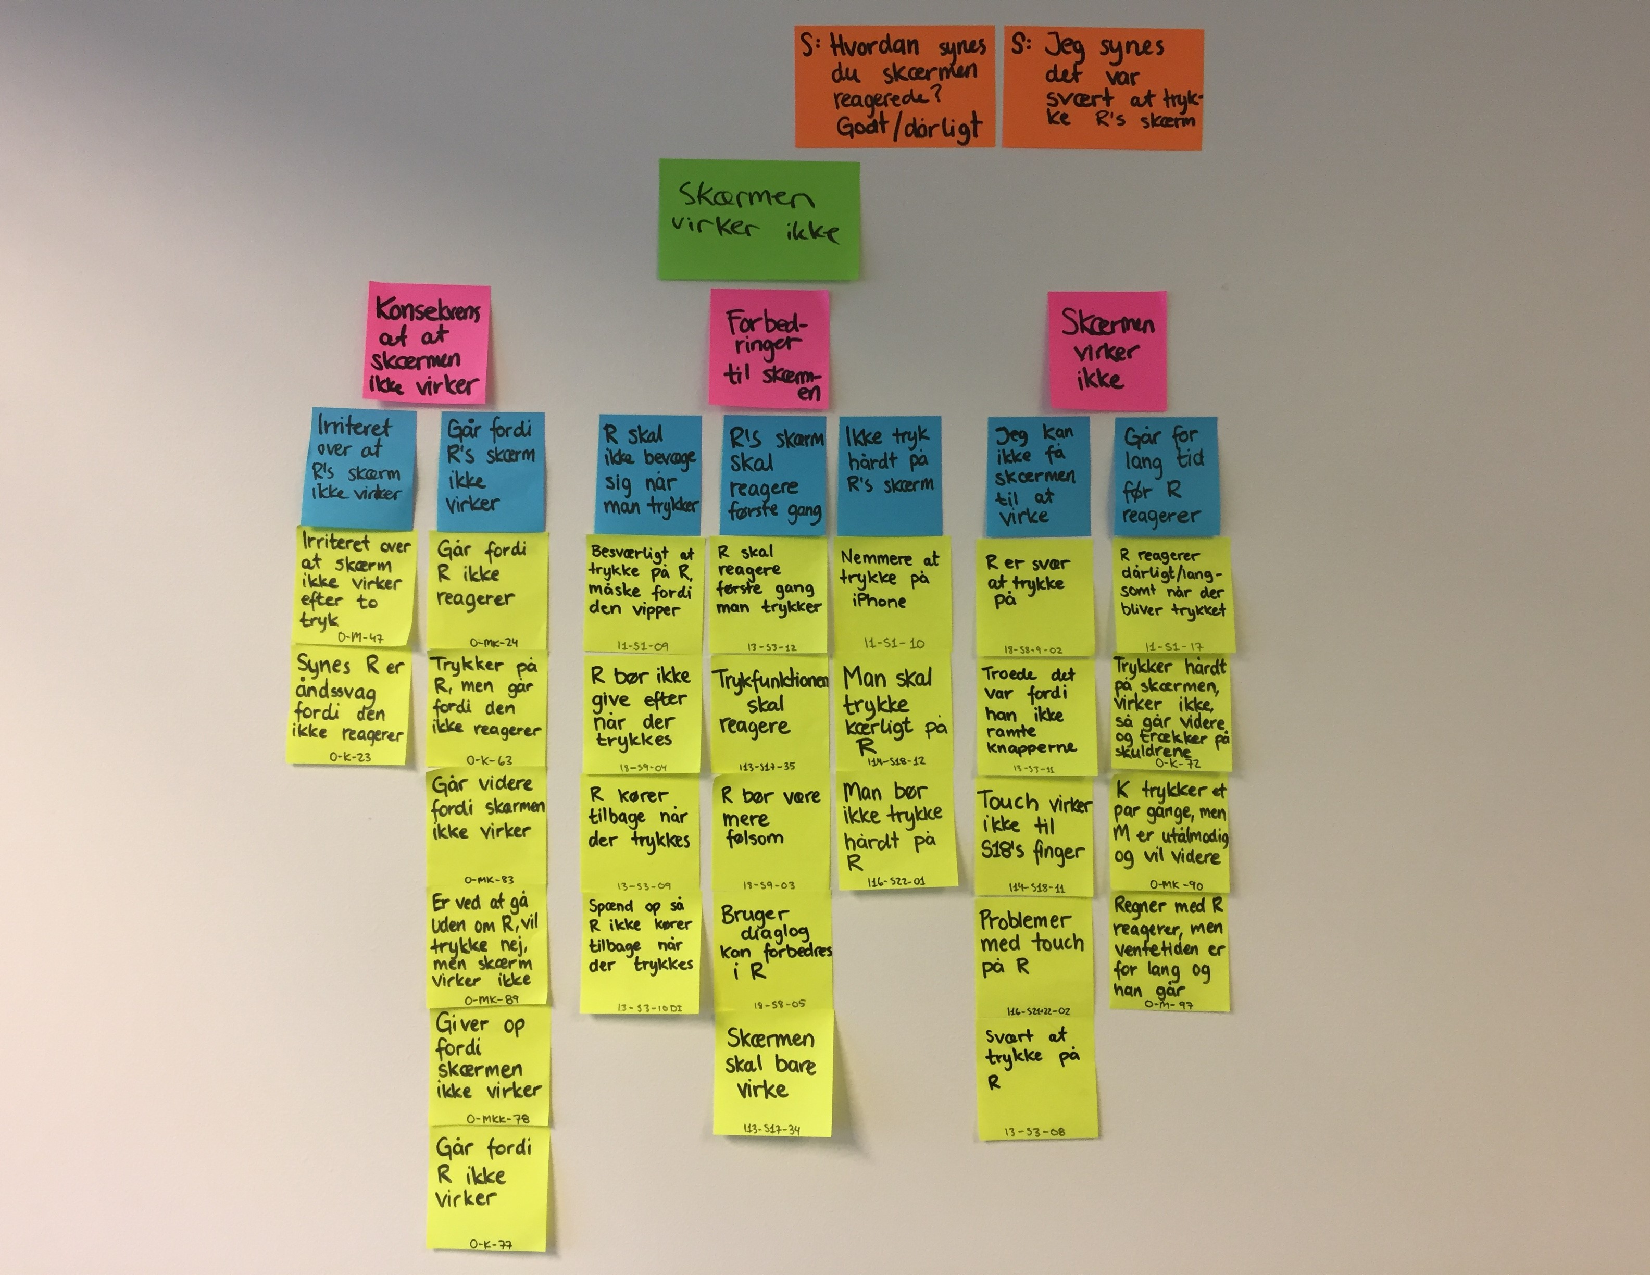
\includegraphics[width = 0.9\textwidth]{Figure/AffinityDiagram/SkaermenVirkerIkke} 
\caption{Oversigt over pink, blå og gule \textit{sticky notes} under den overordnede kategori ``Skærmen virker ikke`` samt de udledte parametre på orange \textit{sticky notes}.}
\label{fig:AFSkaermVirkerIkke}
\end{figure}
\noindent
%
S: Jeg synes det var svært at trykke på R's skærm\\
S: Jeg synes skærmen reagerede dårligt\\
S: Jeg synes skærmen reagerede.. (Dårligt/Godt)
%
\subsection{R kan assistere mennesker}
%
\begin{figure}[H]
\centering
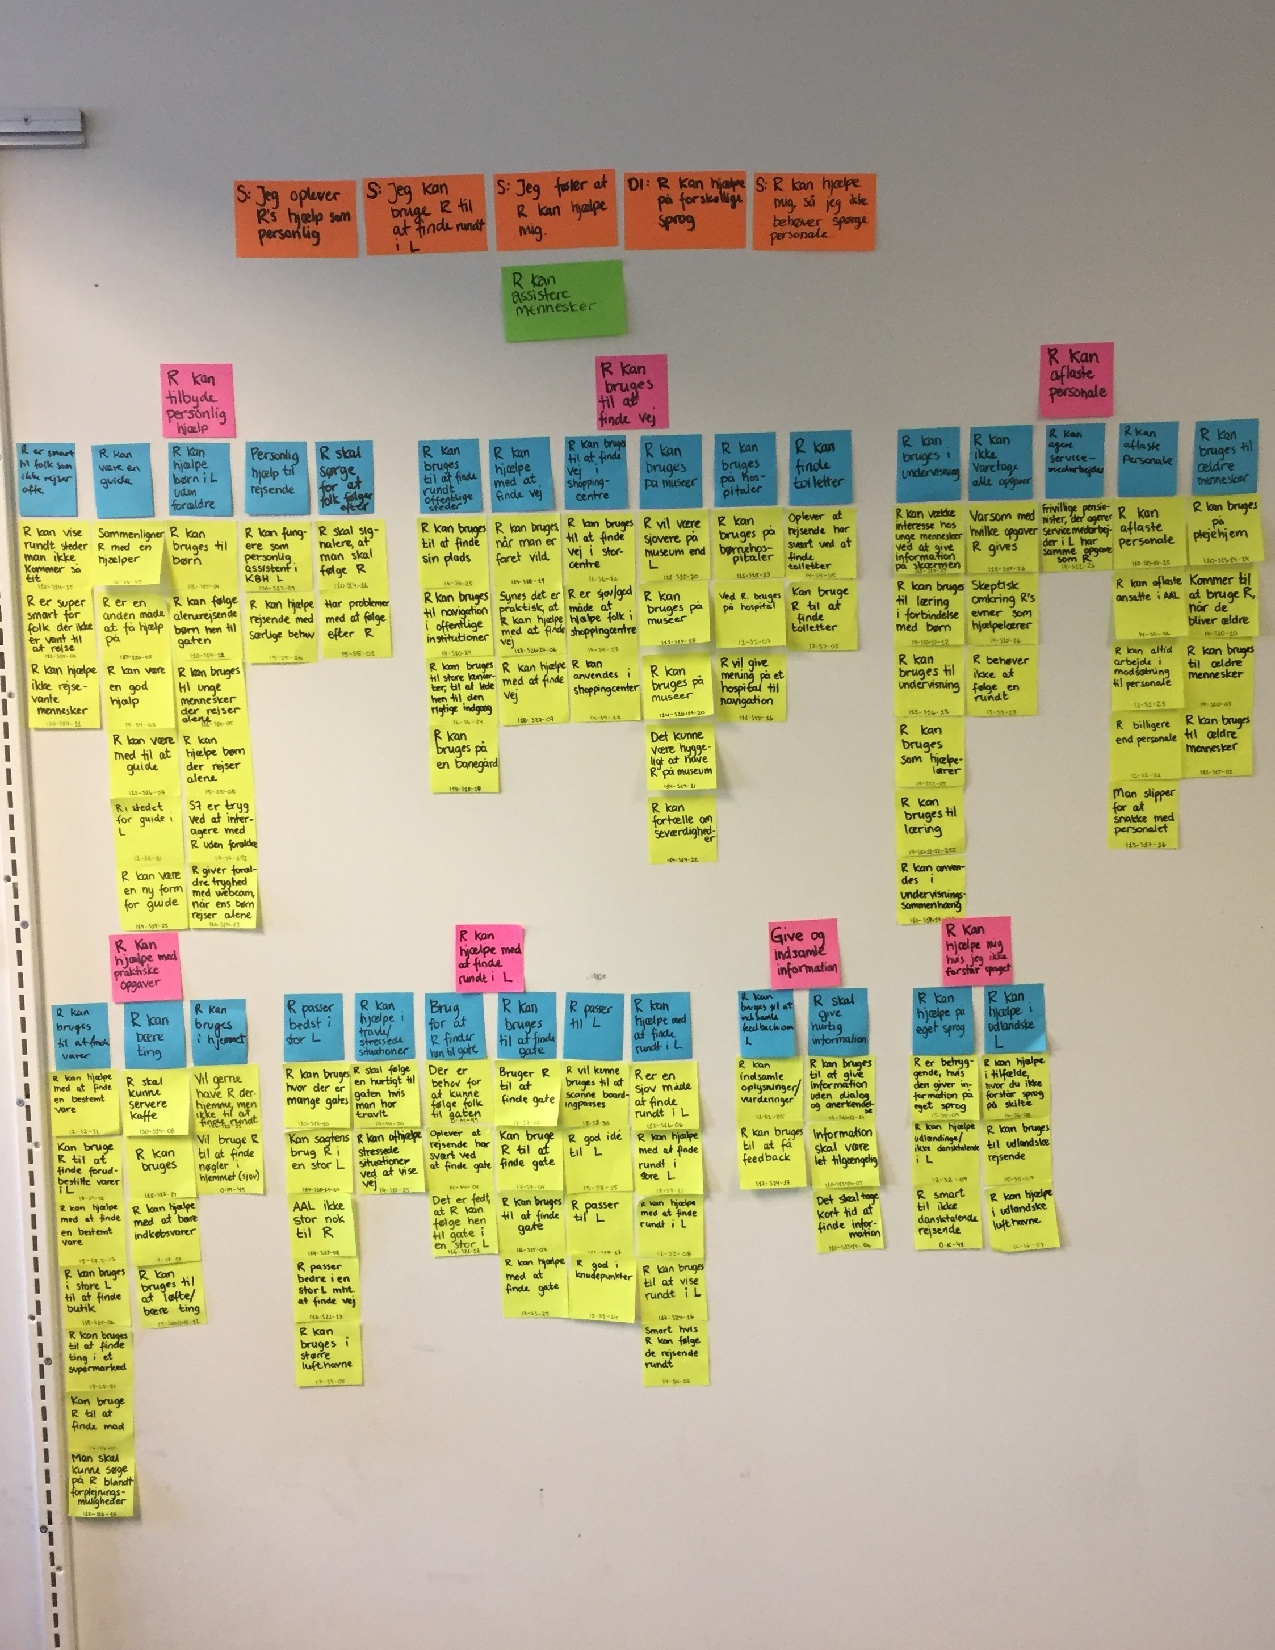
\includegraphics[width = 0.9\textwidth]{Figure/AffinityDiagram/RKanAssistereMennesker} 
\caption{Oversigt over pink, blå og gule \textit{sticky notes} under den overordnede kategori ``R kan assistere mennesker`` samt de udledte parametre på orange \textit{sticky notes}.}
\label{fig:AFRKanAssistereMennesker}
\end{figure}
\noindent
%
S: Jeg kan bruge R til at finde rundt i en lufthavn\\
S: Jeg føler at R kan hjælpe mig\\
S: R kan hjælpe mig så jeg ikke behøver at spørge personale\\
S: Jeg oplever R's hjælp som personlig\\
DI (Design idé): Kan hjælpe i situationer hvor jeg ikke forstår sproget. 

\subsection{R's væremåde}
%
\begin{figure}[H]
\centering
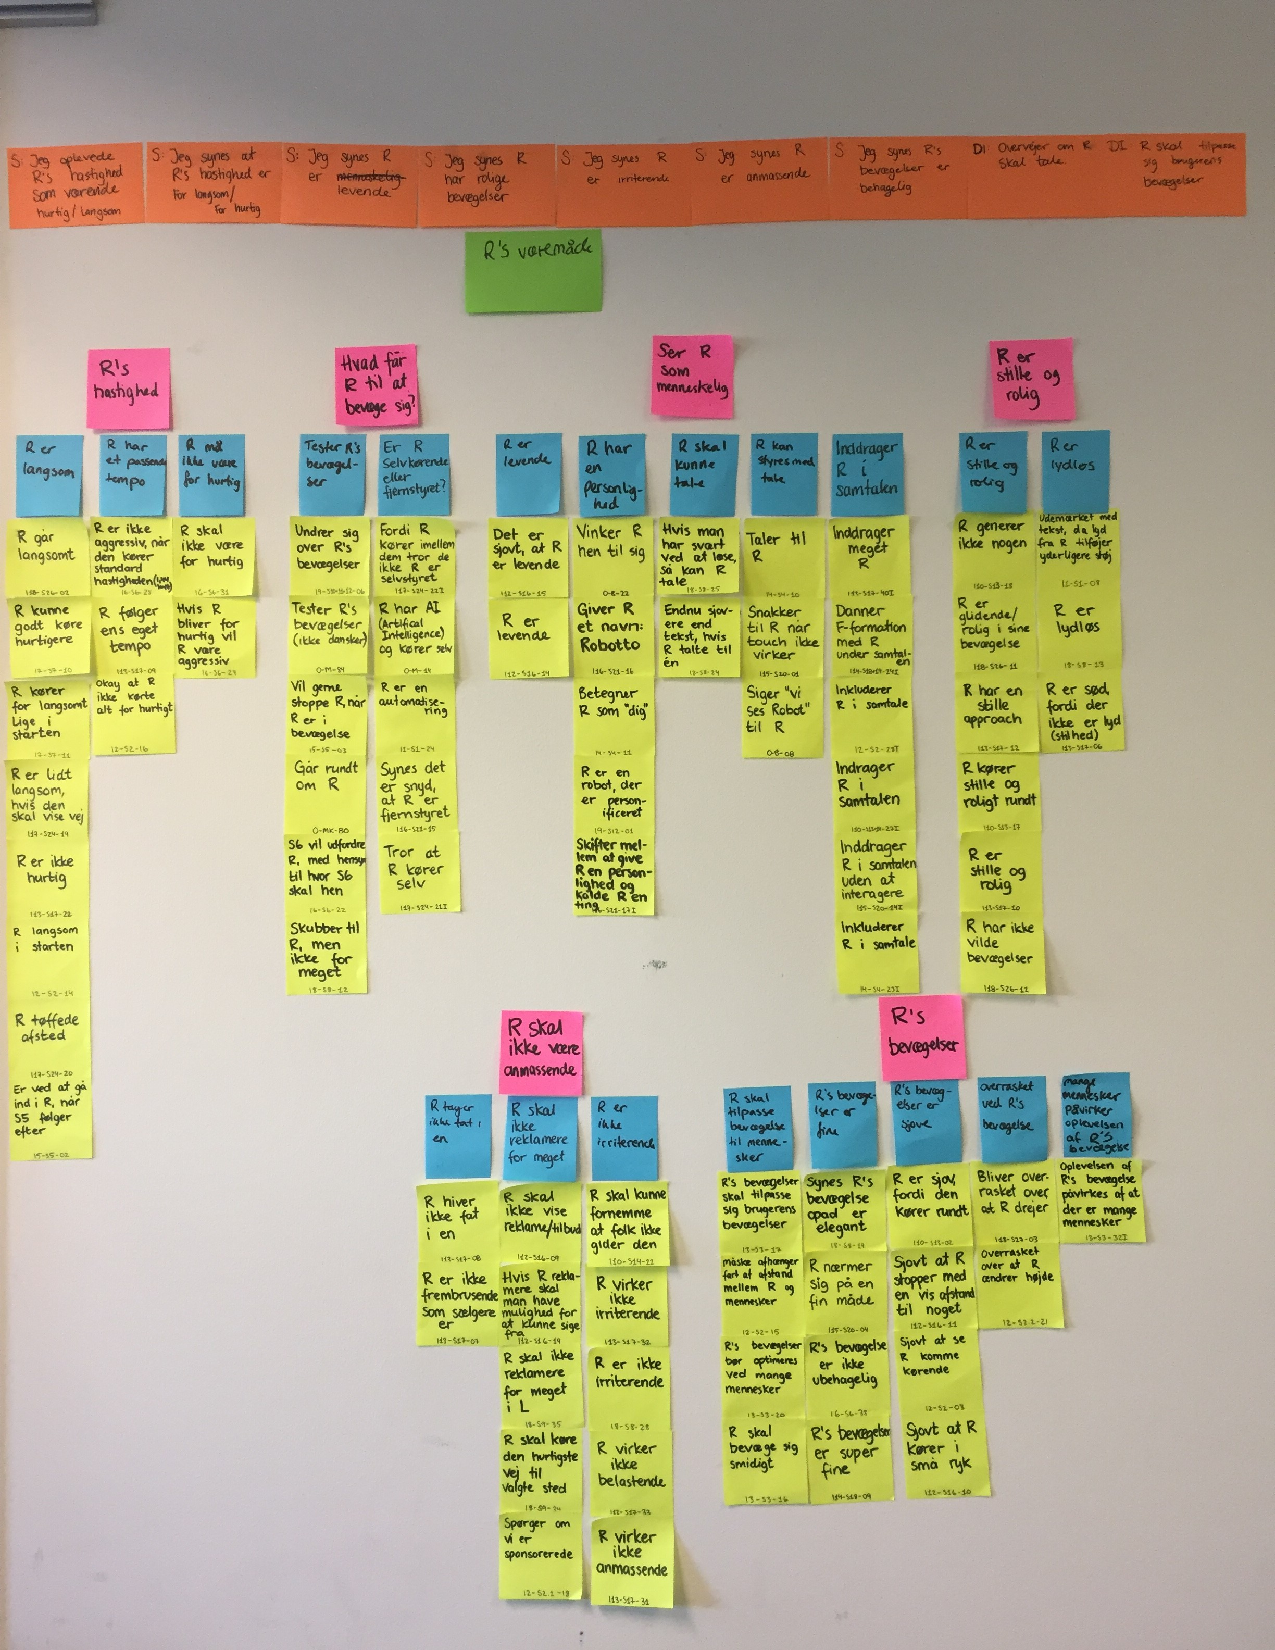
\includegraphics[width = 0.9\textwidth]{Figure/AffinityDiagram/RsVaeremaade} 
\caption{Oversigt over pink, blå og gule \textit{sticky notes} under den overordnede kategori ``R's væremåde`` samt de udledte parametre på orange \textit{sticky notes}.}
\label{fig:AFRsVaeremaade}
\end{figure}
\noindent
%
S: Jeg oplevede R's hastighed som værende.. (Meget langsom/Meget hurtig)\\
S: Jeg synes at R's hastighed er.. (For langsom/For hurtig)\\
S: Jeg synes at R er levende\\
S: Jeg synes at R har rolige bevægelser\\
S: Jeg synes at R er irriterende\\
S: Jeg synes at R er anmassende\\
S: Jeg synes at R's bevægelser er behagelige\\
DI: R skal tilpasse sig brugerens bevægelser\\
DI: Overvej om R skal tale

\subsection{Henvendelse}
%
\begin{figure}[H]
\centering

\includegraphics[width = 0.9\textwidth]{Figure/AffinityDiagram/Henvendelse} 
\caption{Oversigt over pink, blå og gule \textit{sticky notes} under den overordnede kategori ``Henvendelse`` samt de udledte parametre på orange \textit{sticky notes}.}
\label{fig:AFHenvendelse}
\end{figure}
\noindent
%
S: Jeg blev overrasket over R's henvendelse\\
S: Jeg synes at R stod i vejen\\
S: Jeg foretrækker at R henvender sig til mig\\
S: Jeg foretrækker at jeg henvender mig til R\\
S: Jeg synes at R er imødekommende\\
S: Jeg synes at R kom for tæt på\\
S: Jeg synes at R er intimiderende\\
DI: Er skal vende fronten mod den person, som R vil henvende sig til\\
DI: R skal være tæt på den person, som R henvender sig til\\

\subsection{R's udseende}
%
\begin{figure}[H]
\centering
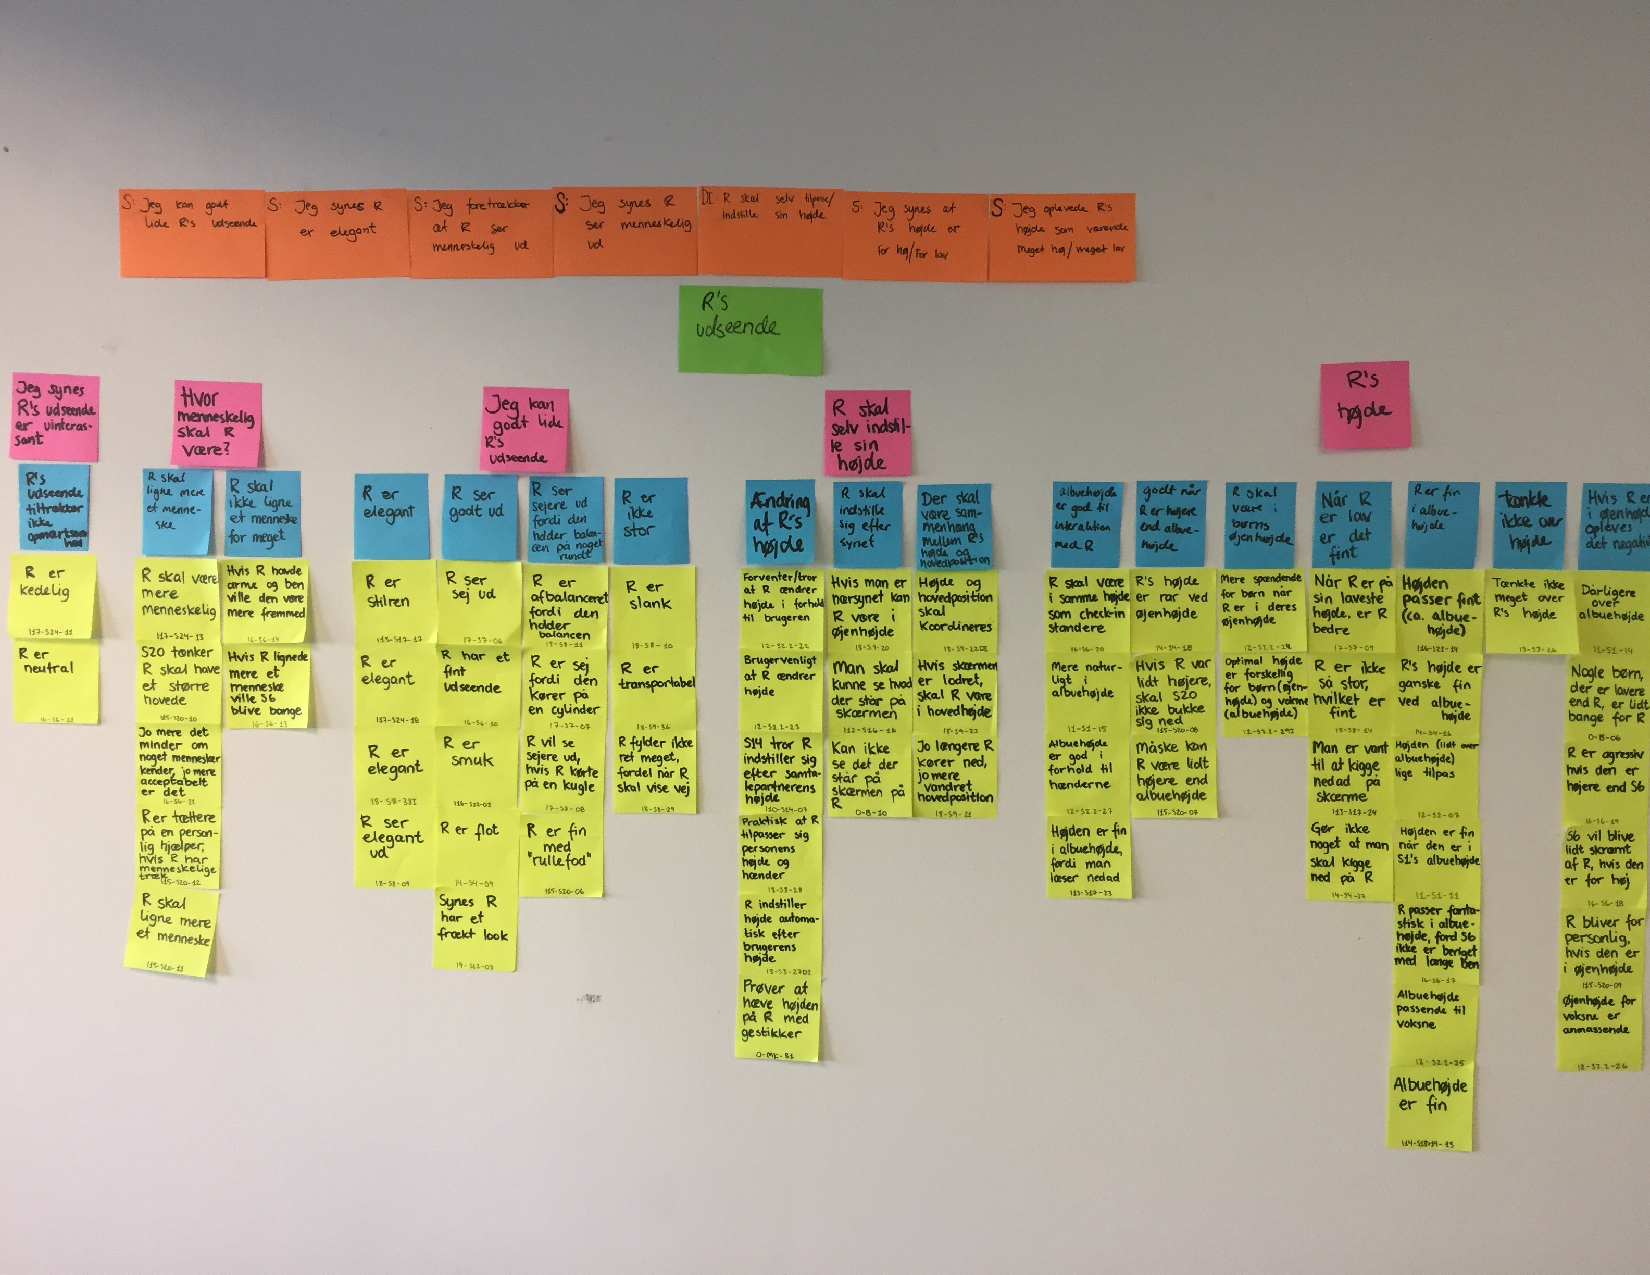
\includegraphics[width = 0.9\textwidth]{Figure/AffinityDiagram/RsUdseende} 
\caption{Oversigt over pink, blå og gule \textit{sticky notes} under den overordnede kategori ``R's udseende`` samt de udledte parametre på orange \textit{sticky notes}.}
\label{fig:AFRsUdseende}
\end{figure}
\noindent
%
S: Jeg synes at R ser menneskelig ud (slet ikke menneskelig/alt for menneskelig)\\
S: Jeg foretrækker at R ser menneskelig ud\\
S: Jeg synes at R er elegant\\
S: Jeg kan godt lide R's udseende\\
S: Jeg oplevede R's højde som værende... (Meget lav/Meget høj)\\
S: Jeg synes at R's højde er...(For lav/For høj)\\
DI: R skal selv indstille/tilpasse sin højde efter brugeren\\

\subsection{Interesse for R}
%
\begin{figure}[H]
\centering
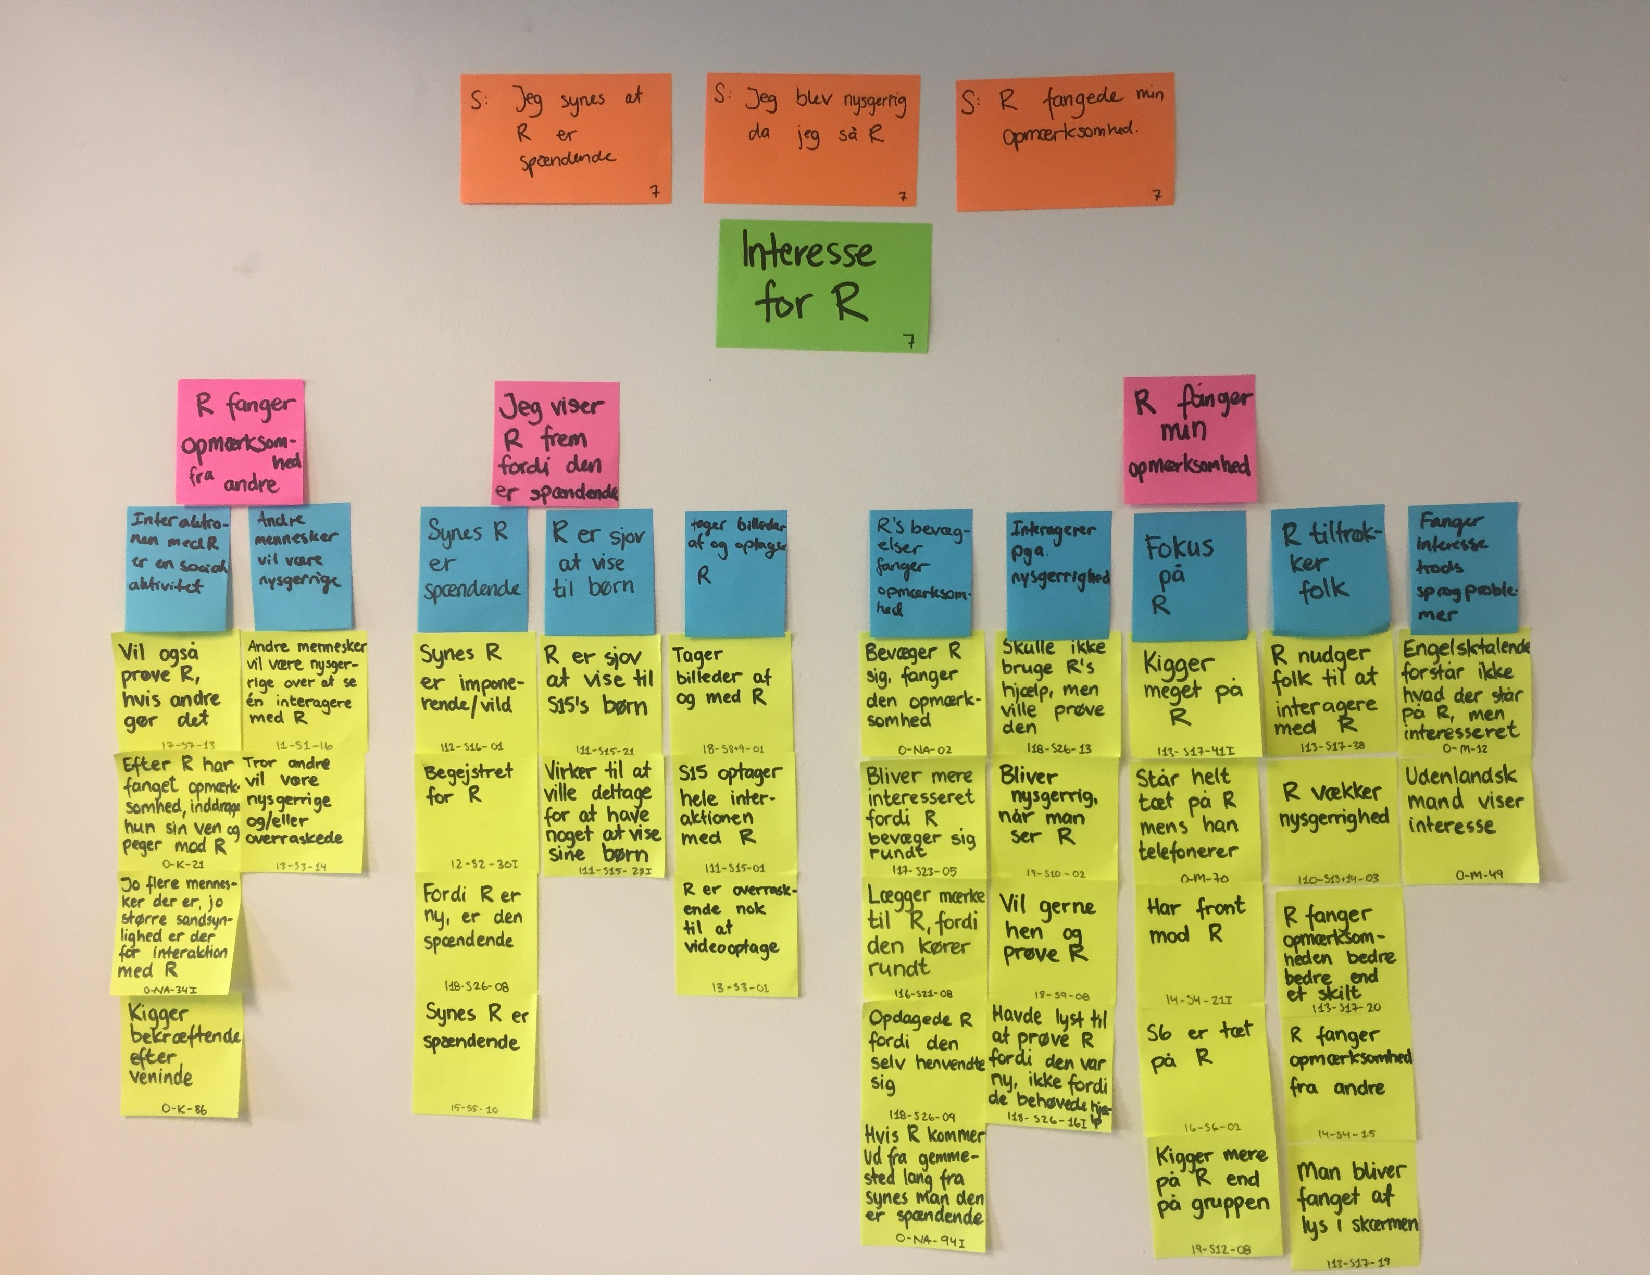
\includegraphics[width = 0.9\textwidth]{Figure/AffinityDiagram/InteresseForR} 
\caption{Oversigt over pink, blå og gule \textit{sticky notes} under den overordnede kategori ``Interesse for R`` samt de udledte parametre på orange \textit{sticky notes}.}
\label{fig:AFInteresseForR}
\end{figure}
\noindent
%
S: R fangede min opmærksomhed\\
S: Jeg blev nysgerrig da jeg så R\\
S: Jeg synes at R er spændende

\subsection{Positiv overfor R}
%
\begin{figure}[H]
\centering
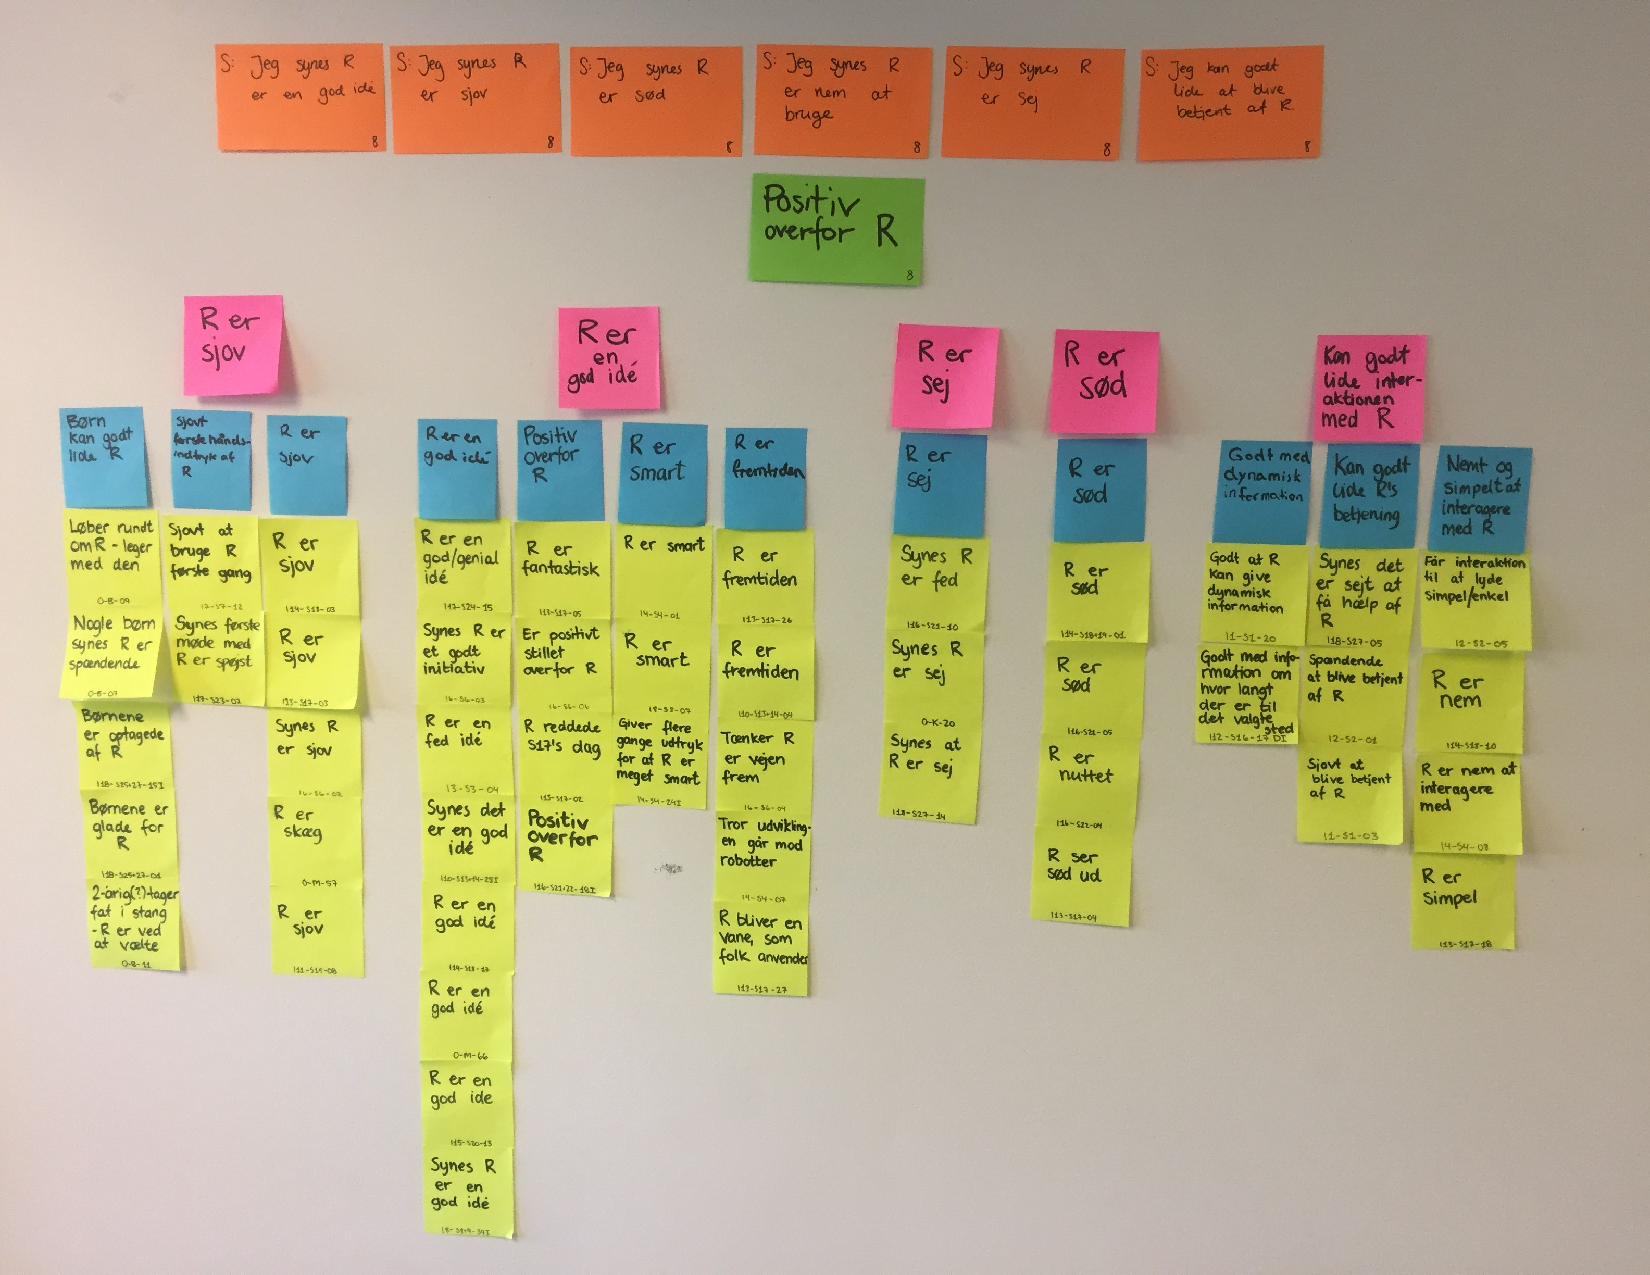
\includegraphics[width = 0.9\textwidth]{Figure/AffinityDiagram/PositivOverforR} 
\caption{Oversigt over pink, blå og gule \textit{sticky notes} under den overordnede kategori ``Positiv overfor R`` samt de udledte parametre på orange \textit{sticky notes}.}
\label{fig:AFPositivOverforR}
\end{figure}
\noindent
%
S: Jeg synes R er sjov\\
S: Jeg synes R er sød\\
S: Jeg synes R er sej\\
S: Jeg synes R er nem at bruge\\
S: Jeg kan godt lide at blive betjent af R\\
S: Jeg synes R er en god idé

\subsection{Kendskab til teknologi}
%
\begin{figure}[H]
\centering
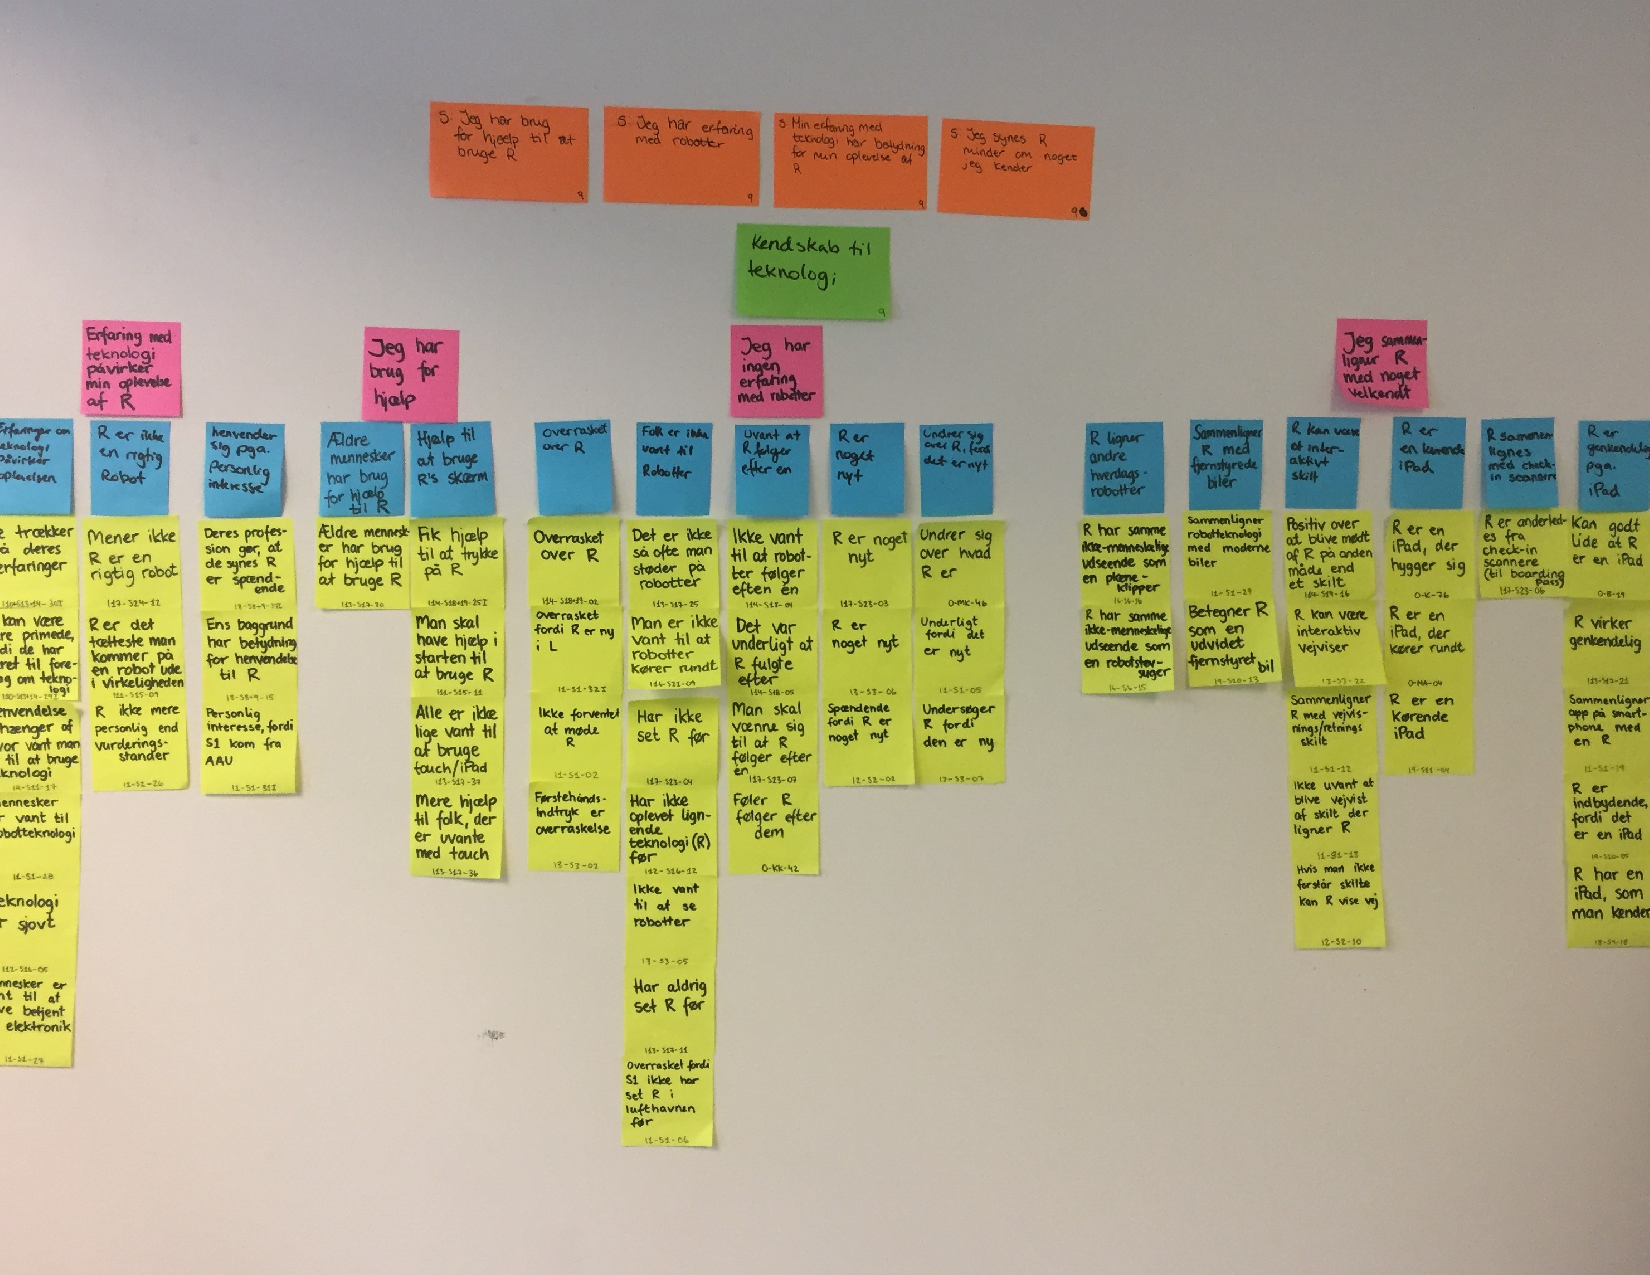
\includegraphics[width = 0.9\textwidth]{Figure/AffinityDiagram/KendskabTilTeknologi} 
\caption{Oversigt over pink, blå og gule \textit{sticky notes} under den overordnede kategori ``Kendskab til teknologi`` samt de udledte parametre på orange \textit{sticky notes}.}
\label{fig:AFKendskabTilTeknologi}
\end{figure}
\noindent
%
S: Jeg har erfaring med robotter\\
S: Jeg har brug for hjælp til at bruge R\\
S: Jeg synes R minder om noget jeg kender\\
S: Min erfaring med teknologi har betydning for min oplevelse af R

\subsection{Tillid til R}
%
\begin{figure}[H]
\centering
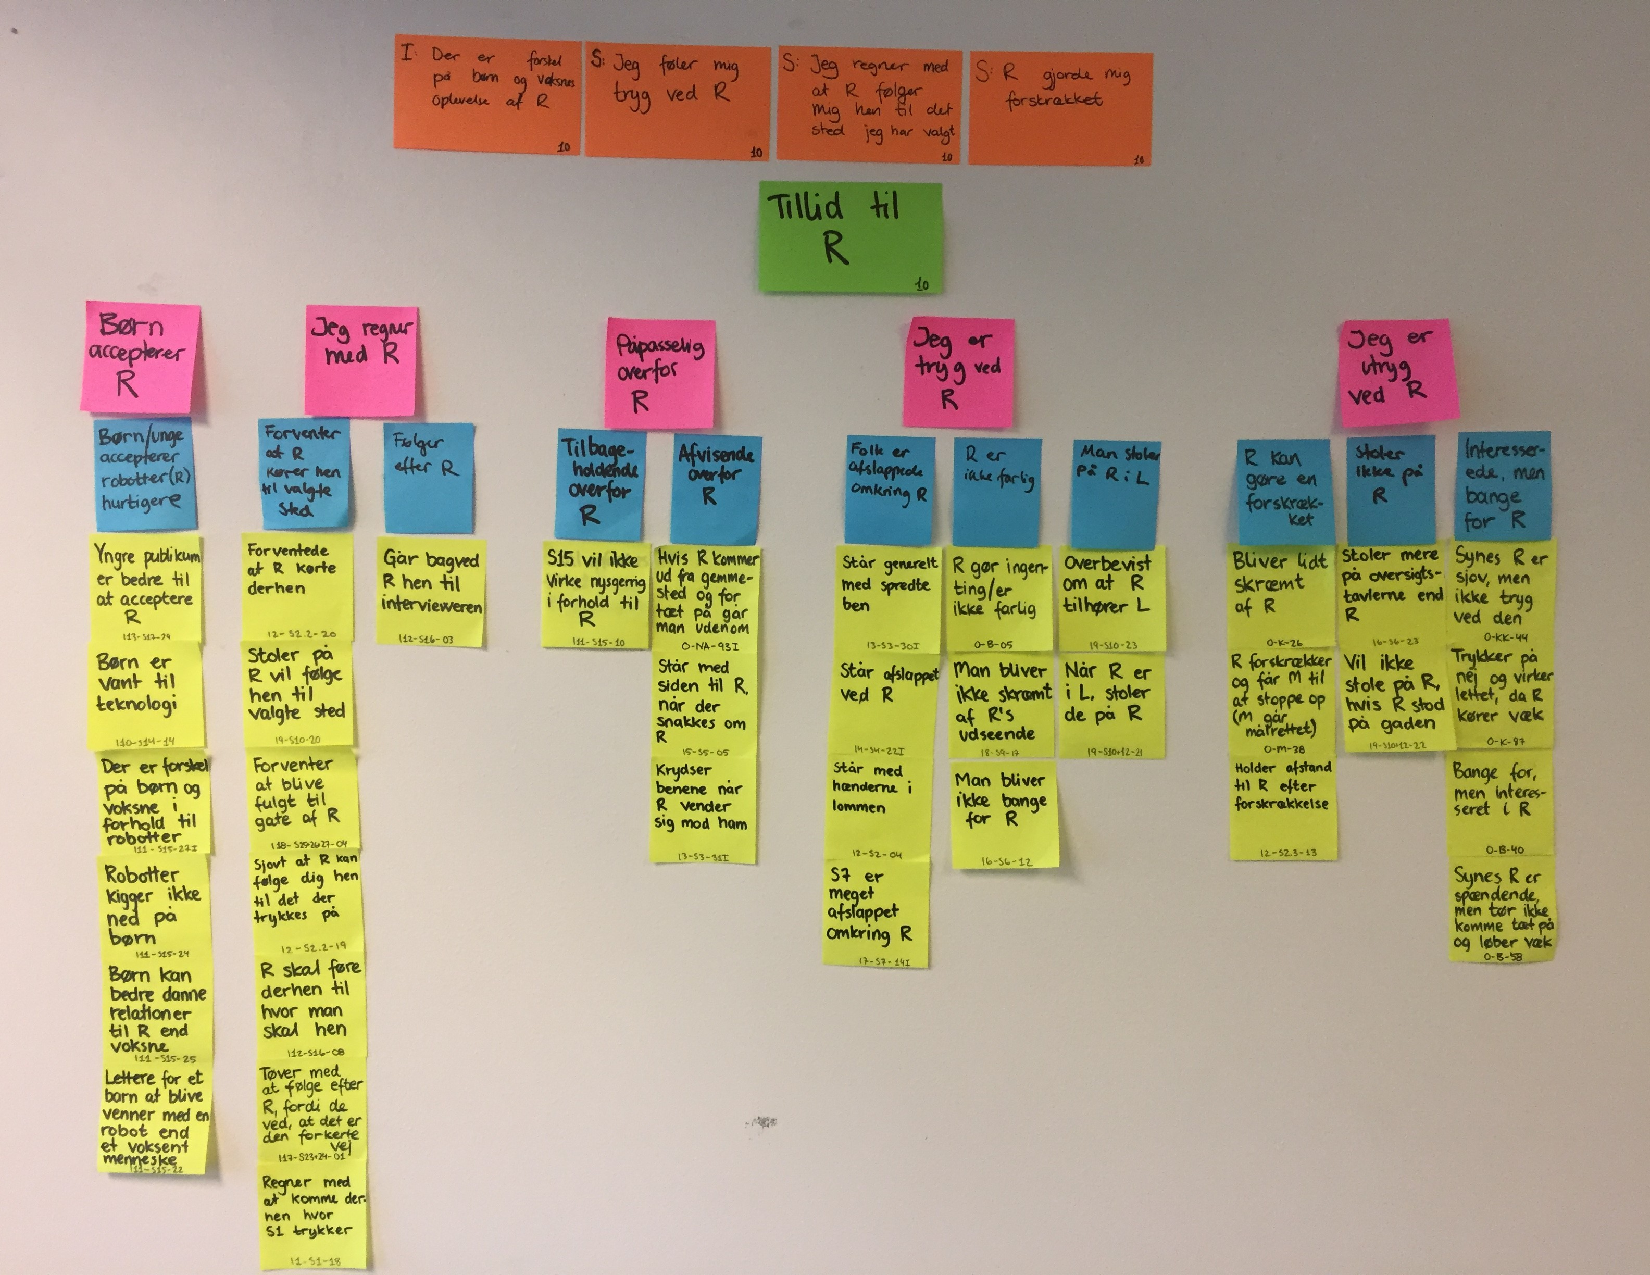
\includegraphics[width = 0.9\textwidth]{Figure/AffinityDiagram/TillidTilR} 
\caption{Oversigt over pink, blå og gule \textit{sticky notes} under den overordnede kategori ``Tillid til R`` samt de udledte parametre på orange \textit{sticky notes}.}
\label{fig:AFTillidTilR}
\end{figure}
\noindent
%
S: Jeg føler mig tryg ved R\\
S: Jeg regner med at R følger mig hen til det sted jeg har valgt\\
S: R gjorde mig forstrækket\\
I: Der er forskel på børn og voksnes oplevelse af R